\chapter{Durchführung}
In diesem Kapitel wird auf die Durchführung der Messungen mit dem Passivradar eingegangen. Dabei wird erläutert werden, wo sich die Quelle des verwendeten Signals befindet und nach welchen Kriterien der Messpunkt ausgewählt wurde und welcher Messpunkt ausgewählt wurde. Außerdem wird der gesamte fertige Messaufbau dargestellt.
\section{Punkt des Signals}
Der Sender unseres Signals ist der Stuttgarter Fernsehturm, dieser liegt im Süden von Stuttgart und ist in Abbildung~\ref{fig:Fernsehturm} zusehen. Das Signal wird vom Stuttgarter Fernsehturm in Richtung der A8 ausgesendet. Hier wird 5G benutzt im Rahmen eines Projektes von einem Zusammenschluss aus Südwestrundfunk (SWR), Kathrein Broadcast GmbH,  DFMG  Deutsche Funkturm GmbH, Porsche AG, Rohde \& Schwarz GmbH \& Co. KG, TU Braunschweig, Telekom Deutschland GmbH. Das Ziel des Projektes ist es die Nutzung von 5G Broadcast für Anwendungen in Fahrzeugen zu erproben. Dafür werden drei Services übertragen: Zwei Fernsehe Programme, die ARD/SWR Mediathek und ein Reiseführer~\cite{5GMAG2020}.
\begin{figure}
    \centering
    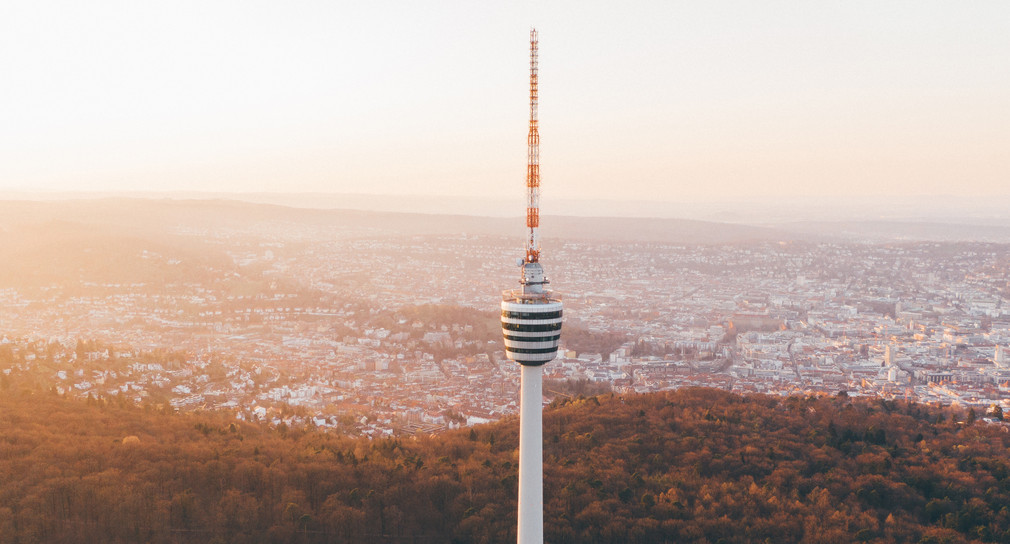
\includegraphics[width=\textwidth]{images/Fernsehturm.jpg}
    \caption{Stuttgarter Fernsehturm}\label{fig:Fernsehturm}
\end{figure}

\section{Messpunkt}
Der Messpunkt ist so gewählt das sowohl der Stuttgarter Flughaffen als auch der Stuttgarter Fernsehturm für das Radar sichtbar sind und außerdem gut vom Studentenwohnheim Geschwister-Scholl-Str. gut erreichbar war. Das Passivradar wurde in der Nähe des Segelflughafen Esslingen aufgebaut, die genaue Position ist in Abbildung~\ref{fig:Einflugschneise} und in Abbildung~\ref{fig:Maps} auf Google Maps erkennen.

\begin{figure}
    \centering
    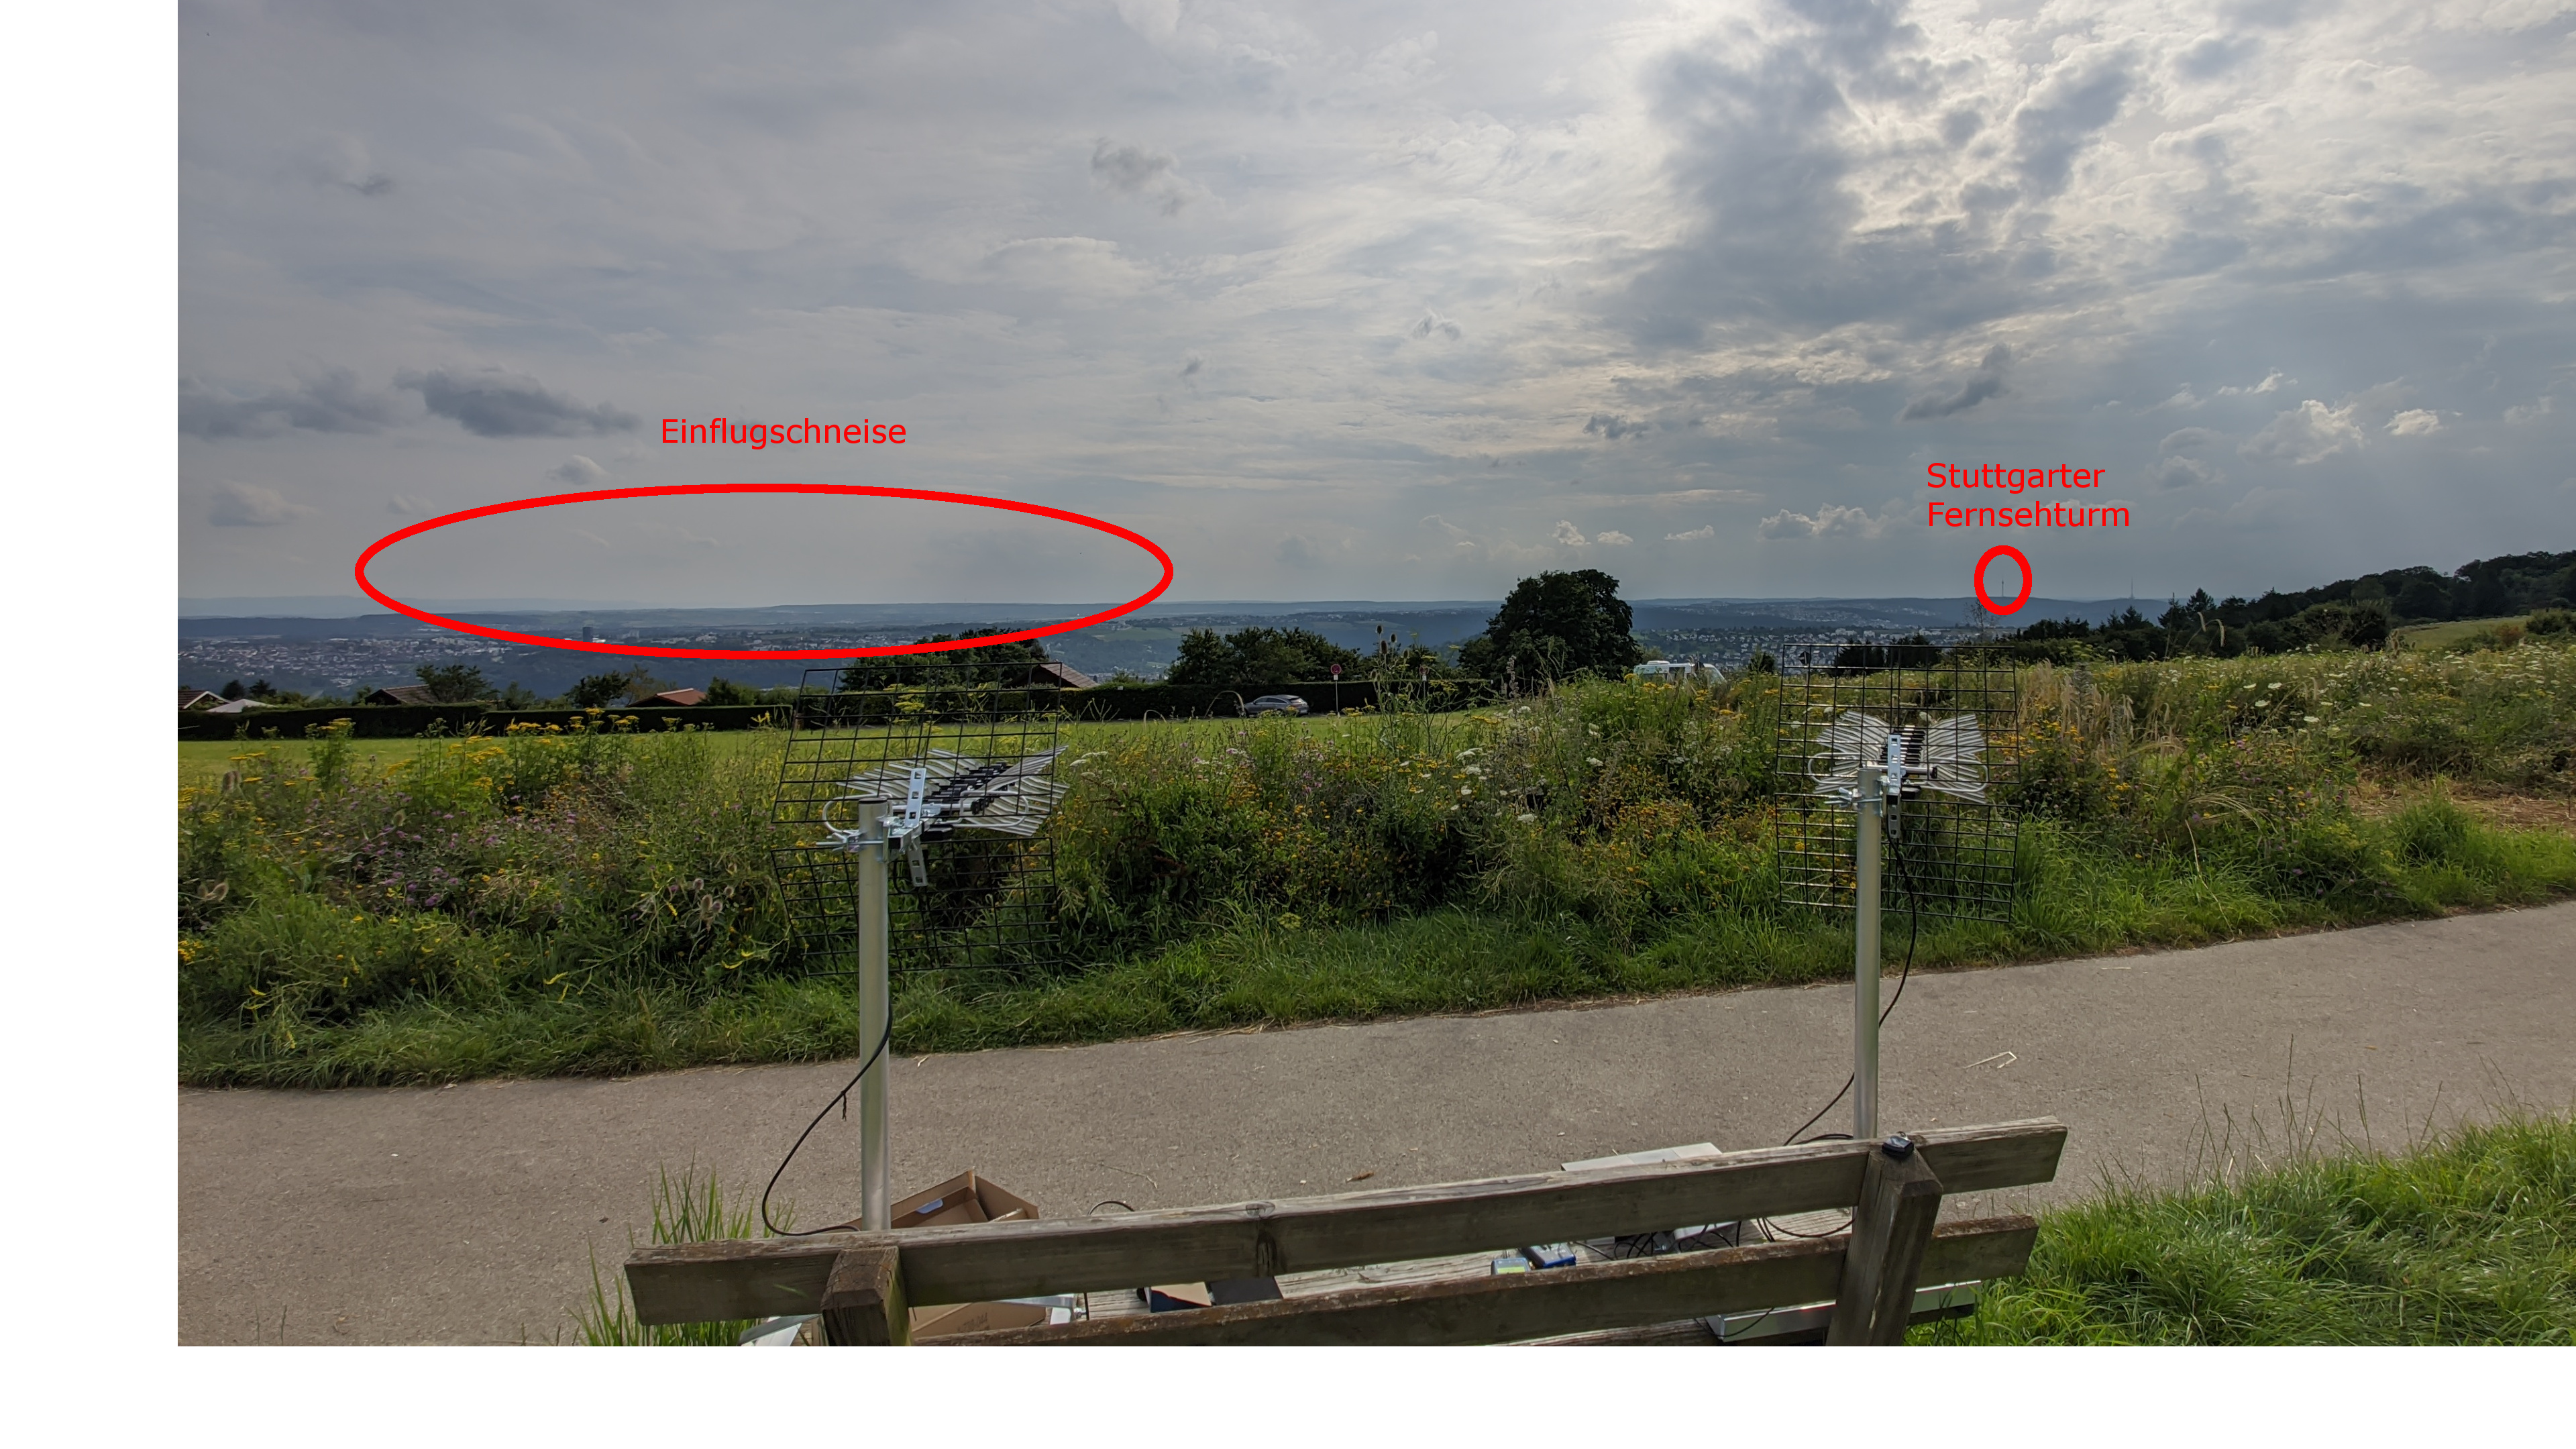
\includegraphics[width=\textwidth]{images/Einflugschneise.jpg}
    \caption{Einflugschneise und Stuttgart Fernsehturm}\label{fig:Einflugschneise}
\end{figure}

\begin{figure}
    \centering
    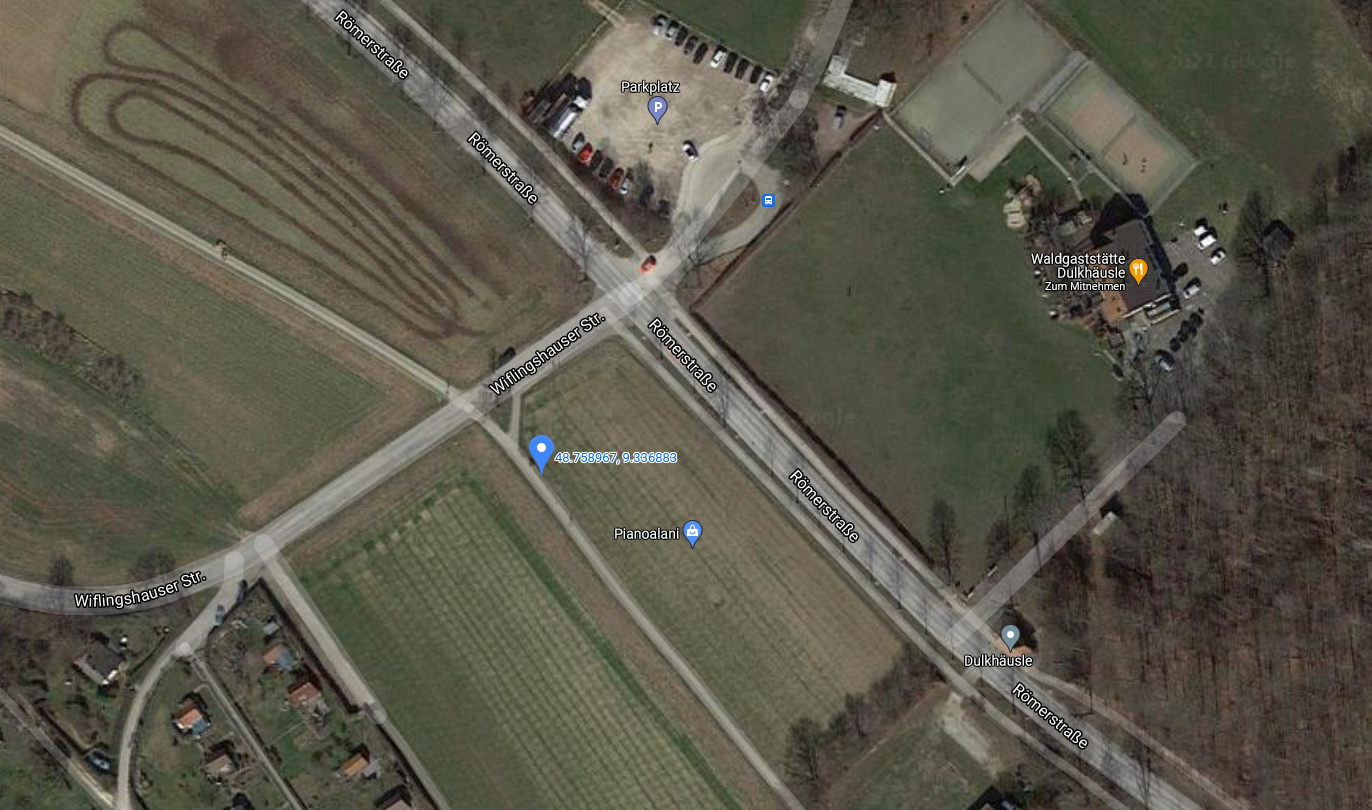
\includegraphics[width=\textwidth]{images/Maps_Messpunkt.png}
    \caption{Possition des Messpunkt}\label{fig:Maps}
\end{figure}

\section{Messaufbau}
Der Messaufbau besteht aus den Komponenten die im Kapitel~\ref{sct:setup} auf S.\pageref{sct:setup} erläutert wurden. Der gesamte fertige Aufbau ist dann in Abbildung~\ref{fig:Messaufbau} zu sehen hier werden die beiden SDRs~\ref{sct:sdr} sowie der OCXO Oscillator~\ref{sct:Oscillator} mit einem Laptop mit SDR-angel Sofware verbunden. Die Antennen sind so ausgerichtet, dass eine auf den Stuttgarter Flughafen ausgerichtet ist und die andere auf den Stuttgarter Fernsehturm.

\begin{figure}
    \centering
    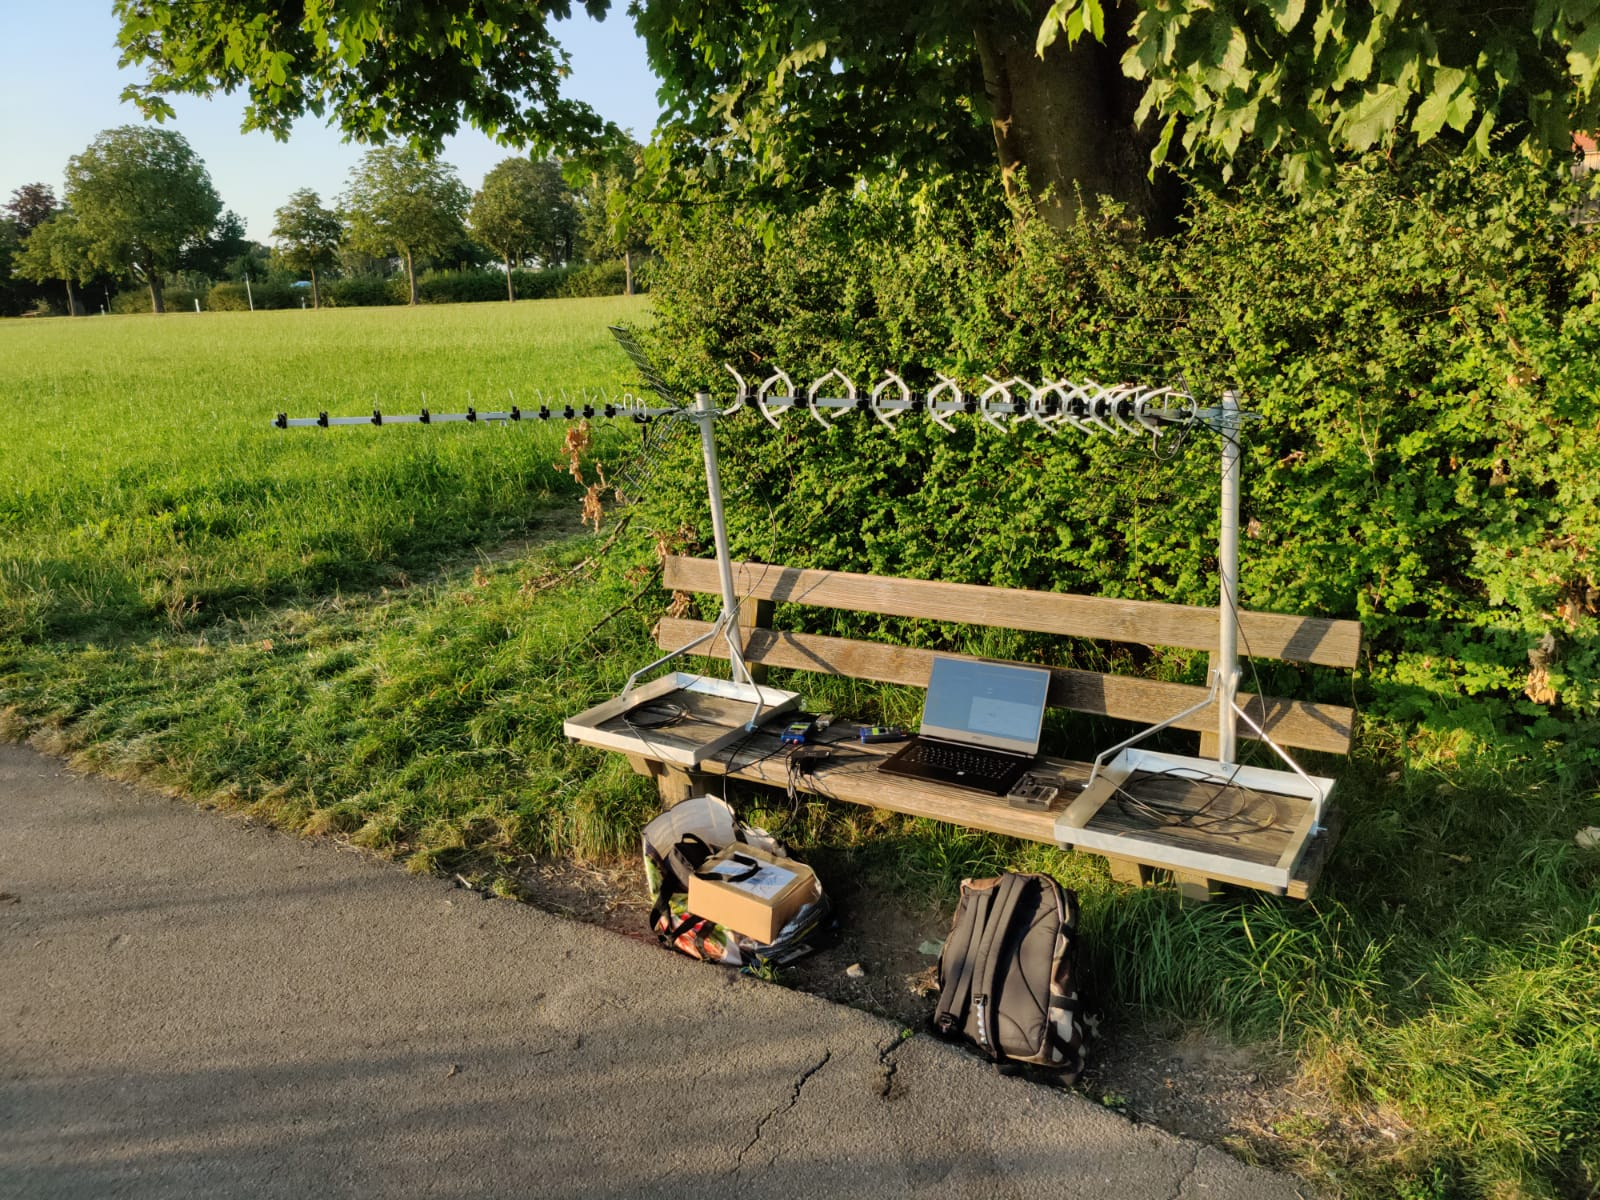
\includegraphics[width=\textwidth]{images/Messaufbau.jpg}
    \caption{Aufbau der Messung}\label{fig:Messaufbau}
\end{figure}
